\section{Introduction}
\label{sec:parikshan-intro}
\begin{figure*}[ht!]
	\begin{center}
		%    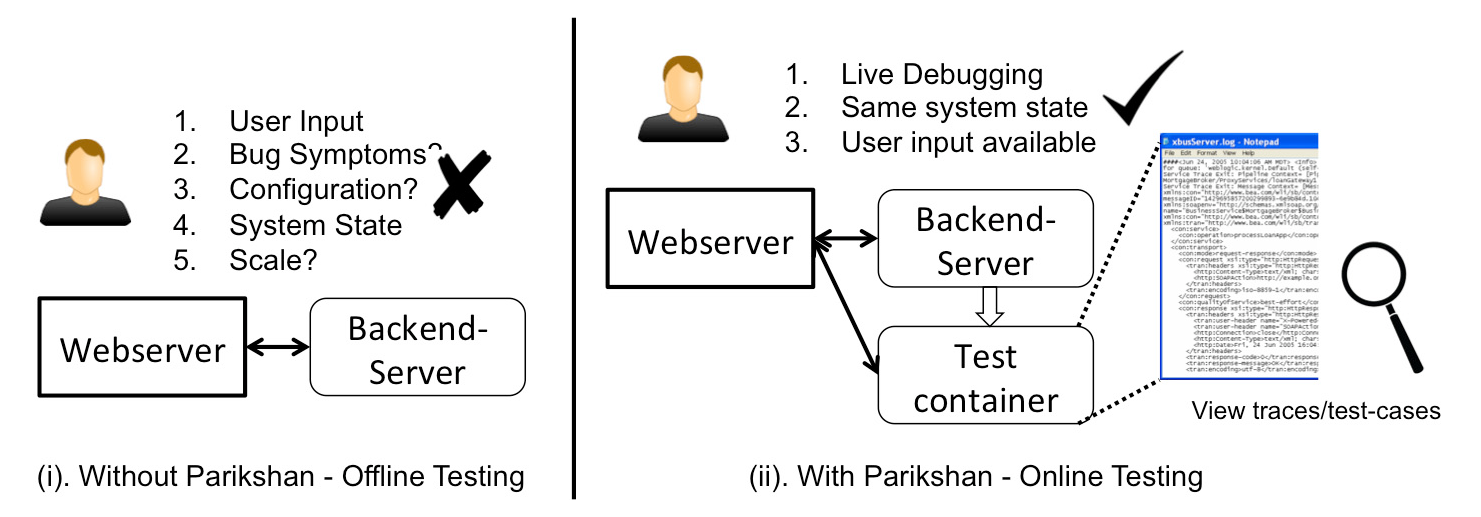
\includegraphics[width=0.7\textwidth]{figs/motivation.eps}
		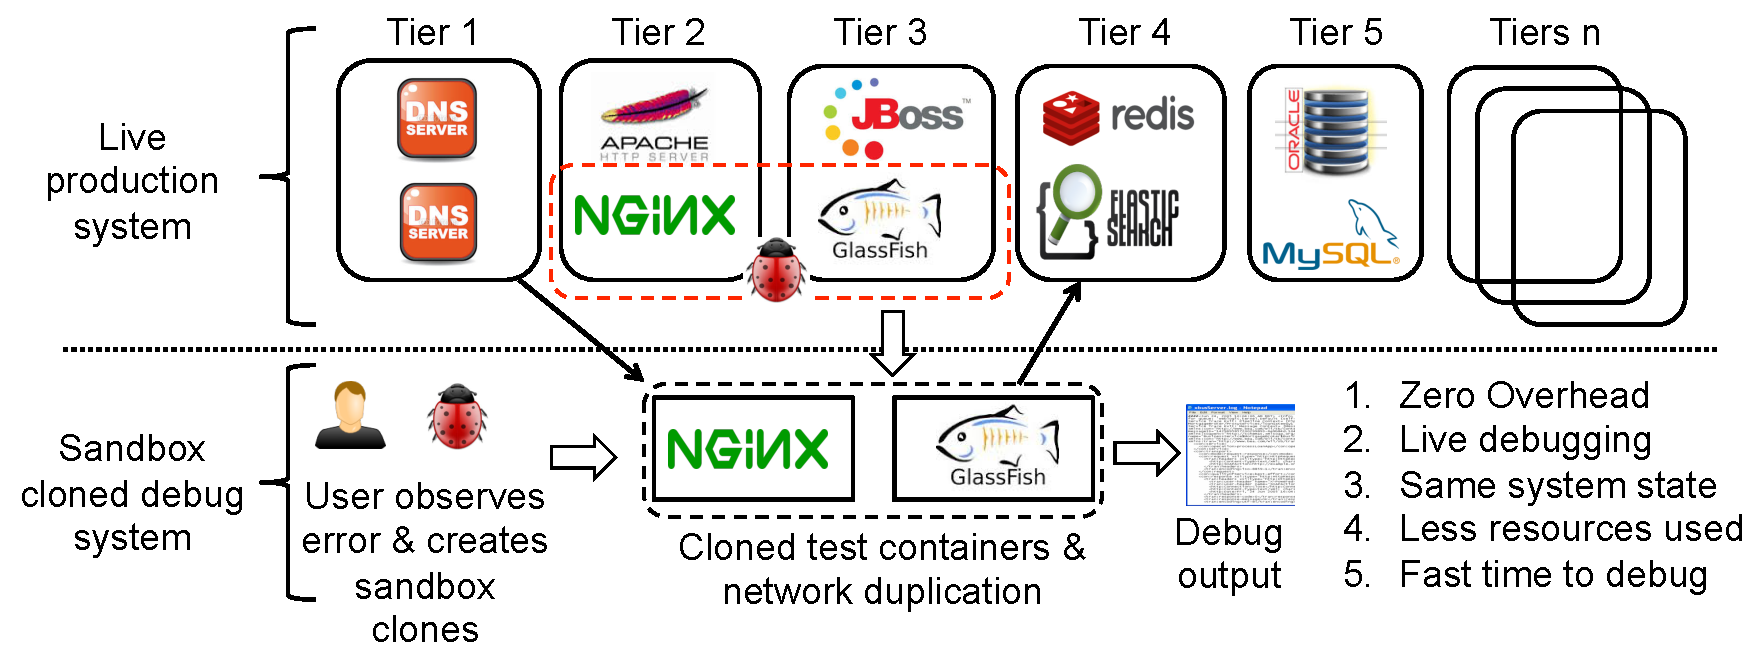
\includegraphics[width=0.9\textwidth]{parikshan/figs/workflow3.pdf}
		\caption{Workflow of \parikshan in a live multi-tier production system with several interacting services. When the administrator of the system observes errors in two of it's tiers, he can create a sandboxed clone of these tiers and observe/debug them in a sandbox environment without impacting the production system.}
		\label{fig:motivation}
	\end{center}
\end{figure*}

Rapid resolution of incident (error/alert) management~\cite{sasase2013} in online service-oriented systems~\cite{microservice-book,hdfs,cassandra,redis} is extremely important.
The large scale of such systems means that any downtime has significant financial penalties for all parties involved.
However, the complexities of virtualized environments coupled with large distributed systems have made bug localization extremely difficult.
Debugging such production systems requires careful re-creation of a similar
environment and workload, so that developers can reproduce and identify the cause of the problem.

Existing state-of-art techniques for monitoring production systems rely on execution trace information. 
These traces can be replayed in a developer's environment, allowing them to use dynamic instrumentation and debugging tools to understand the fault that occurred in production.
On one extreme, these monitoring systems may capture only very minimal, high
level information, for instance, collecting existing log information and
building a model of the system and its irregularities from it~\cite{magpie,fay,failuresketching,problemsolvingSysTap}. \xxx{get more cites here too}
While these systems impose almost no overhead on the production system being
debugged (since they simply collect log information already being collected, or
have light-weight monitoring), they are limited in their fault finding and redproduction power, hence limited in their utility to developers.
On the other extreme, some monitoring systems capture complete execution traces, allowing the entire application execution to be exactly reproduced in a debugging environment \cite{odr,revirt,laadan2010transparent,geels2007friday}.
Despite much work towards minimizing the amount of such trace data captured, overheads imposed by such tracing can still be unacceptable for production use: in most cases, the overhead of tracing is at least 10\%, and it can balloon up to 2-10x overhead. \cite{pinplay,drdebug}.

We seek to allow developers to diagnose and resolve crashing and non-crashing failures of production service-oriented systems \emph{without suffering any performance overhead}.
Our key insight is that for most service-oriented systems, a failure can be reproduced simply by replaying the network inputs passed to the application.
For these failures, capturing very low-level sources of non-determinism (e.g. thread scheduling or general system calls, often with very high overhead) is unnecessary to successfully and automatically reproduce the buggy execution in a development environment.
We evaluated this insight by studying 16 real-world bugs (see Section~\ref{sec:casestudy}), which we were able to trigger by only duplicating and replaying network packets.
Furthermore, we categorized 217 bugs from three real world applications, finding that most were similar in nature to the 16 that we reproduced, suggesting that our approach would be applicable to them as well (see Section~\ref{sec:survey}).
%TODO - look into PRES to see if we can prove that capturing all sources of non-determinism is not important


Guided by this insight, we have created \parikshan\footnote{\parikshan is the \toolNameLang word for  testing}, which allows for real-time, online debugging of production services \textbf{\emph{without imposing any performance penalty}}.
At a high level, \parikshan leverages live cloning technology to create a sandboxed replica environment.
This replica is kept isolated from the real world so that developers can modify the running system in the sandbox to support their debugging efforts without fear of impacting the production system.
Once the replica is executing, \parikshan replicates all network inputs flowing to the production system, buffering and feeding them (without blocking the production system) to the debug system.
Within that debug system, developers are free to use heavy-weight instrumentation that would not be suitable in a production environment to diagnose the fault.
Meanwhile, the production system can continue to service other requests.
\parikshan can be seen as very similar to tools such as Aftersight \cite{aftersight} that offload dynamic analysis tasks to replicas and VARAN \cite{Hosek:2015:VUE:2694344.2694390} that support multi-version execution, but differs in that its high-level recording level (network inputs, rather than system calls) allows it to have significantly lower overhead.


%\parikshan primarily focuses on bugs~\cite{Zhang:2013:ADS:2486788.2486830, liu2005mining, kremenek2007factor}.
\parikshan focuses on helping developers debug faults \emph{online} --- as they occur in production systems.
We expect \parikshan to be used in cases of tricky bugs that are highly sensitive to their environment, such as semantic bugs, performance bugs, resource-leak errors, configuration bugs, and concurrency bugs.
Although in principle, \parikshan can be used to diagnose crashing bugs, we target primarily non-crashing bugs, where it is important for the production system to remain running even after a bug is triggered, for instance, to continue to process other requests. 
%For instance, semantic bugs are caused because of logical errors, which lead to an unexpected output, performance bugs result in a slow-down of the application. 
We present a more detailed explanation of these categories in Section~\ref{sec:casestudy}.

%We assume our target system has been deployed based on micro-service architecture~\cite{microservice-book,microservices}, which advocates running each service in isolation.
We leverage container virtualization technology (e.g., Docker~\cite{docker}, OpenVZ~\cite{openvz}), which can be used to pre-package services so as to make deployment of complex multi-tier systems easier (i.e. DockerHub~\cite{dockerhub,dockerhub_article} provides pre-packaged containers for storage, webserver, database services etc.).
Container based virtualization is now increasingly being used in practice~\cite{containerCloud}.
In contrast to VM's containers run natively on the physical host (i.e. there is no hypervisor layer in between), this means that there is no additional overhead, and near-native performance for containers~\cite{performanceComparisonlxcVM,performanceEvalContainers}.
While \parikshan could also be deployed using VM's, container virtualization is much more light weight in terms of resource usage.

%Essentially, micro-service architecture allows us to launch debug containers which targets one service at a time. 
%This is not a necessary condition, but makes deploying \parikshan easier and more practical.

%We leverage user-space container virtualization technologies (OpenVZ/LXC~\cite{openvz,lxc}).
%For simplicity, we assume that our target systems utilize service-oriented architectures, where each service (application, DNS, indexing, storage) is sandboxed in separate containers (\texttt{OpenVZ}~\cite{openvz}).
%This allows us to launch debug containers, which can target one application component at a time.
%While our techniques can also be applied to traditional VMs, containers are lighter-weight and use far fewer resources.

\noindent
The key benefits of our system are:
\begin{itemize}[leftmargin=*,topsep=0pt,itemsep=-1ex,partopsep=1ex,parsep=1ex]
\item \textbf{Zero Overhead Monitoring:} While existing approaches have focused on minimizing the recording overhead. 
\parikshan uses novel non-blocking network duplication to avoid any overhead at all in the production environment.	
\item \textbf{Sandbox debugging:} \parikshan provides a cloned sandbox environment to debug the production application.
This allows a safe mechanism to diagnose the error, without impacting the functionality of the application.
\item \textbf{Capture large-scale context:} Allows capturing the context of large scale production systems, with long running applications. Under normal circumstances capturing such states is extremely difficult as they need a long running test input and large test-clusters.
%\item \textbf{Short time-to-debug:} These techniques contribute to a shortened debug time, by allowing debuggers to directly gather trace data, without needing to bring down the system. 
\end{itemize}

\noindent
The rest of the paper is organized as follows.
In Section~\ref{sec:motivation}, we describe a motivating scenario.
Section~\ref{sec:design} and \ref{sec:implementation} describe the design and implementation of \parikshan and each of it's internal components.
We then present a case study of 16 real-world bugs successfully reproduced by \parikshan in Section~\ref{sec:casestudy}.
%We have tested \parikshan live network duplication process to re-create 16 production bugs in 5 well-known software systems (MySQL, Apache HTTPD, Redis, Hadoop/HDFS) see section~\ref{sec:casestudy}. 
%Furthermore, we performed a survey of Bugzilla reports of apache and MySQL to show that a majority of bugs in production systems can be classified in 5 categories that can in principle be handled by \parikshan (see section~\ref{sec:survey}).
This is followed by the evaluation in Section~\ref{sec:evaluation}.
In Section~\ref{sec:application}, we discuss potential applications of \parikshan. 
Finally, we discuss some challenges in Section~\ref{sec:threats}, give some related work in Section~\ref{sec:related} and conclude.
